% Gerado por scripts/gerar-figuras-monografia.py; não editar.
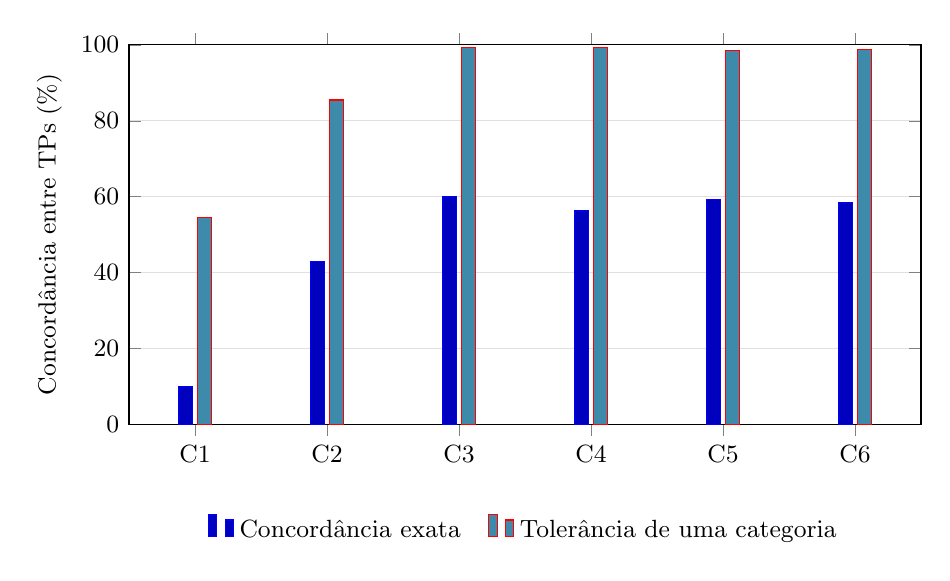
\begin{tikzpicture}
\begin{axis}[
width=0.96\textwidth,height=6.4cm,
tick label style={font=\small},label style={font=\small},
legend style={font=\small,at={(0.5,-0.22)},anchor=north,legend columns=3,draw=none,/tikz/every even column/.append style={column sep=8pt}},
ymajorgrids=true,grid style={black!12},
ybar,bar width=5pt,ymin=0,ymax=100,ylabel={Concordância entre TPs (\%)},xtick={1,2,3,4,5,6},xticklabels={C1,C2,C3,C4,C5,C6},enlarge x limits=0.1,legend columns=2
]
\addplot+[ybar,fill=blue!75!black] coordinates {(1,10.00000000) (2,43.01675978) (3,60.12295990) (4,56.34107541) (5,59.37188406) (6,58.56228956)};
\addlegendentry{Concordância exata}
\addplot+[ybar,fill=cyan!65!black] coordinates {(1,54.61538462) (2,85.47486034) (3,99.30094363) (4,99.33438593) (5,98.50066821) (6,98.82491582)};
\addlegendentry{Tolerância de uma categoria}
\end{axis}
\end{tikzpicture}
